%
\section{Результаты расчетов тестовых задач}
%
В соответствии с описанной математической моделью были проведены расчеты
нескольких тестовых задач, результаты которых качественно верно описывают
рассматриваемые явления. Проверить согласованность результатов расчетов с
экспериментом пока не представляется возможным.

\subsection{Задача о перераспределении фаз}
Рассматриваем область пористой среды, имеющую форму параллелепипеда. Пористость и
абсолютная проницаемость породы постоянны во всем объеме:  $m$=0.4,\; $K=6.64\cdot 10^{-11}$ м$^2$.
Плотности фаз при давлении $P=P_\text{атм}$:\; $\rho_{w0}=1000 \text{кг}/\text{м}^3$,\; 
$\rho_{n0}=850 \text{кг}/\text{м}^3$,\;
$\rho_{g0}=1.4 \text{кг}/\text{м}^3$. 
Коэффициенты вязкости:\; $\mu_w=0.001 \text{Па}\cdot \text{с}$,\;
$\mu_n=0.001 \text{Па}\cdot \text{с}$,\; $\mu_g=1.84\cdot 10^{-5} \text{Па}\cdot \text{с}$.
Коэффициенты сжимаемости жидкостей:\; $\beta_w=4.4\cdot 10^{-7} \text{Па}^{-1}$,\;
$\beta_n=10^{-6} \text{Па}^{-1}$. Во всей области задаем следующее 
начальное распределение:\; $S_w=0.4$,\; $S_n=0.35$,\; $S_g=0.25$, 
$P_w=P_\text{атм}+\rho g h$($h$ - глубина, отсчитывается от верхнего края области). 
Граничную поверхность считаем непроницаемой, что может быть интерпретировано так,
что среда огорожена непроницаемым резервуаром. 

Под действием силы тяжести происходит перераспределение фаз.

Поставленная задача является квазиодномерной. Таким образом, результаты расчетов
могут быть представлены в виде зависимости профилей насыщенностей фаз от времени.

По оси $x$ отложено расстояние по вертикали от дна резервуара. По оси $y$--
значения насыщенностей каждой из фаз на расстоянии $x$ от дна резервуара
в определенный момент расчетного времени. 

\begin{center}
 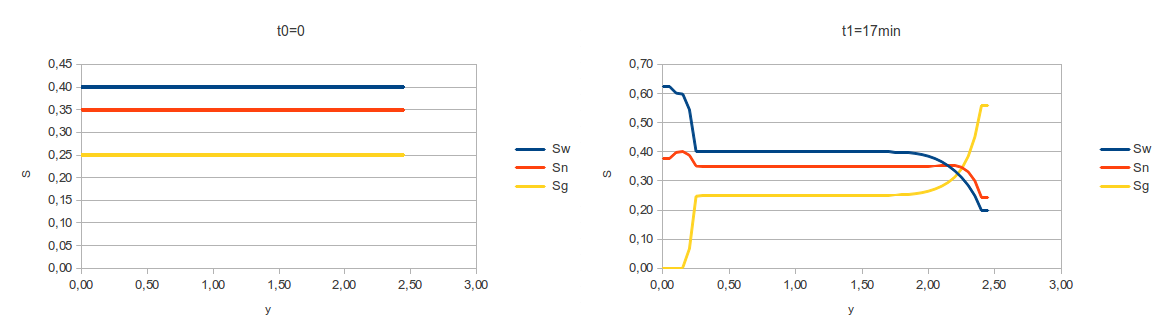
\includegraphics[width=15.5cm,height=5cm]{test1_1}
\end{center}
\begin{center}
 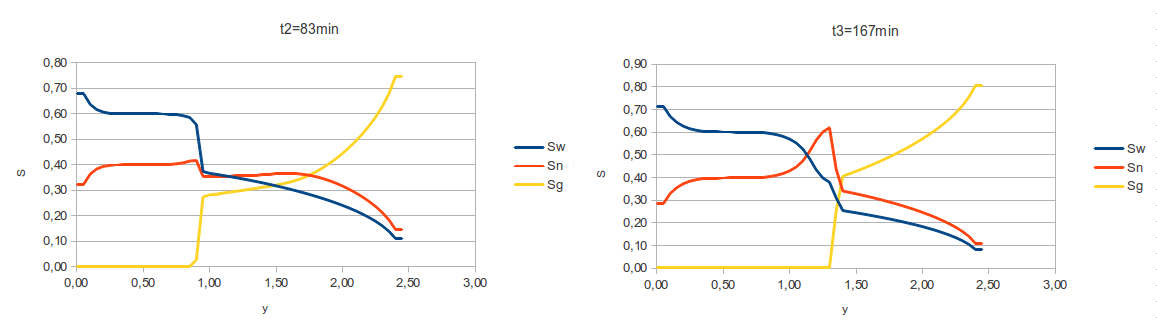
\includegraphics[width=15.5cm,height=5cm]{test1_2}
\end{center}
\begin{center}
 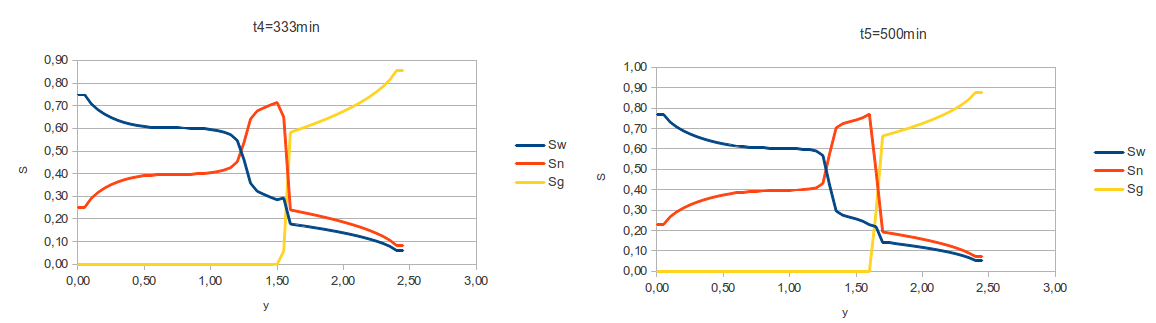
\includegraphics[width=15.5cm,height=5cm]{test1_3}
\end{center}
\begin{center}
 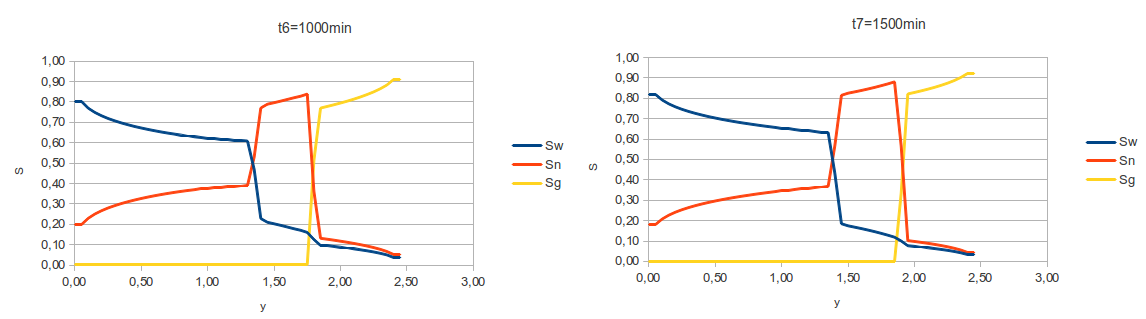
\includegraphics[width=15.5cm,height=5cm]{test1_4}
\end{center}

Таким образом, под действием силы тяжести водная фаза занимает
преимущественно нижнюю часть резервуара, нефтяная -- в основном среднюю
и немного нижнюю, а газовая -- почти целиком верхнюю. Такое распределение
вызвано разницей плотностей фаз и заданными зависимостями относительных
проницаемостей фаз от насыщенностей.

\newpage
\subsection{Задача просачивания с источником на границе}
Расматриваем двумерную область пористой среды, имеющую форму
прямоугольника. Пористость и абсолютная проницаемость породы постоянны во всем
объеме. Параметры модели такие же, как
в первой тестовой задаче.
Во всей области задаем следующее 
начальное распределение: $S_w=0.4$,\; $S_n=0.35$,\; $S_g=0.25$, 
$P_w=P_\text{атм}+\rho g h$($h$ - глубина, отсчитывается от верхнего края области).
Пусть размер области -- $N_x\cdot N_y$.
Граничную поверхность, кроме части верхней границы, считаем непроницаемой, 
что может быть интерпретировано так,
что среда огорожена непроницаемым резервуаром, имеющим сверху отверстие с
координатами: $(N_x/3, N_y)$, $(2N_x/3, N_y)$. Через отверстие происходит обмен веществом между 
резервуаром и окружающей средой. На отверстии заданы условия: $P_w=P_\text{атм}$,

$ \dfrac{\partial S_w}{\partial t}= 
\begin{cases}
 q, \; S_w<S_{max}\\
 0, \; \text{иначе}
\end{cases}
$,
$ \dfrac{\partial S_n}{\partial t}=-q S_n$.

На последующих рисунках изображена динамика изменения насыщенностей 
фаз. Слева направо цветом изображены значения насыщенностей $S_w$, $S_n$, $S_g$, соответственно, 
в зависимости от координат в разное время.

\begin{center}
 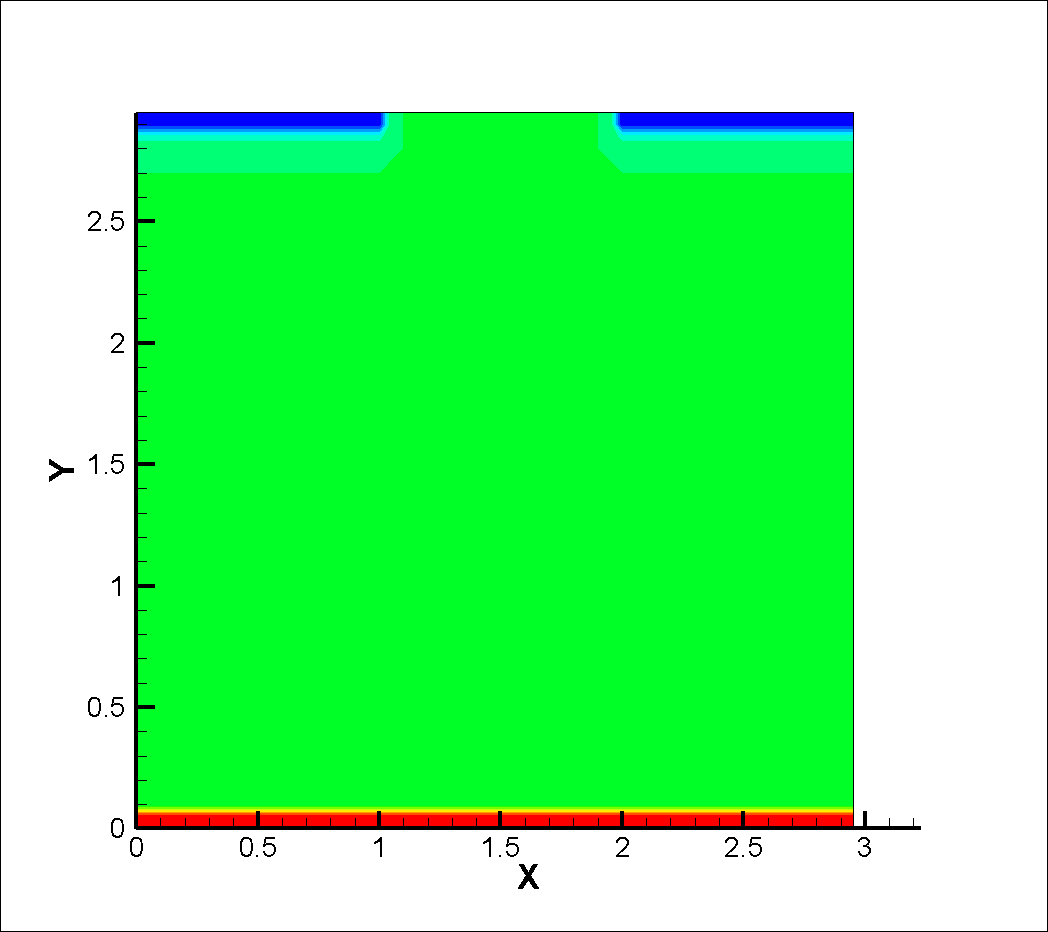
\includegraphics[width=5cm,height=5cm]{test2_1Sw}
 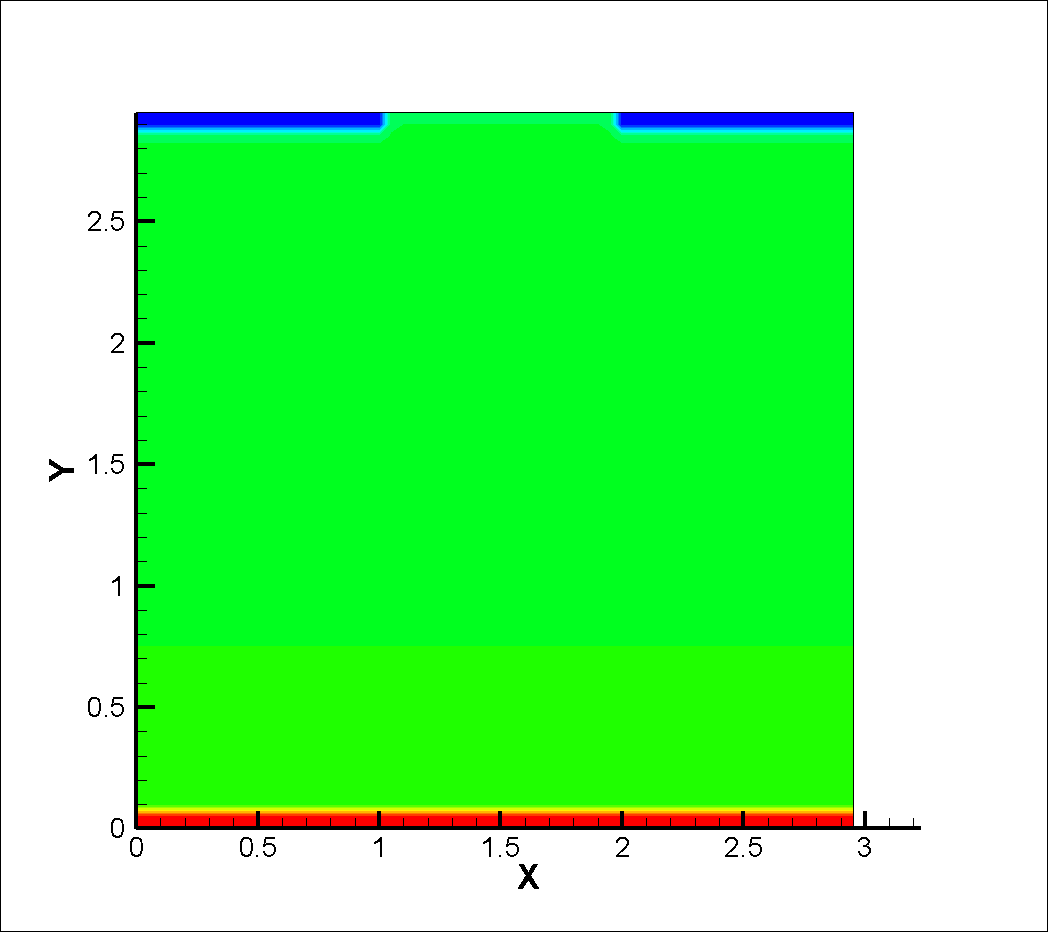
\includegraphics[width=5cm,height=5cm]{test2_1Sn}
 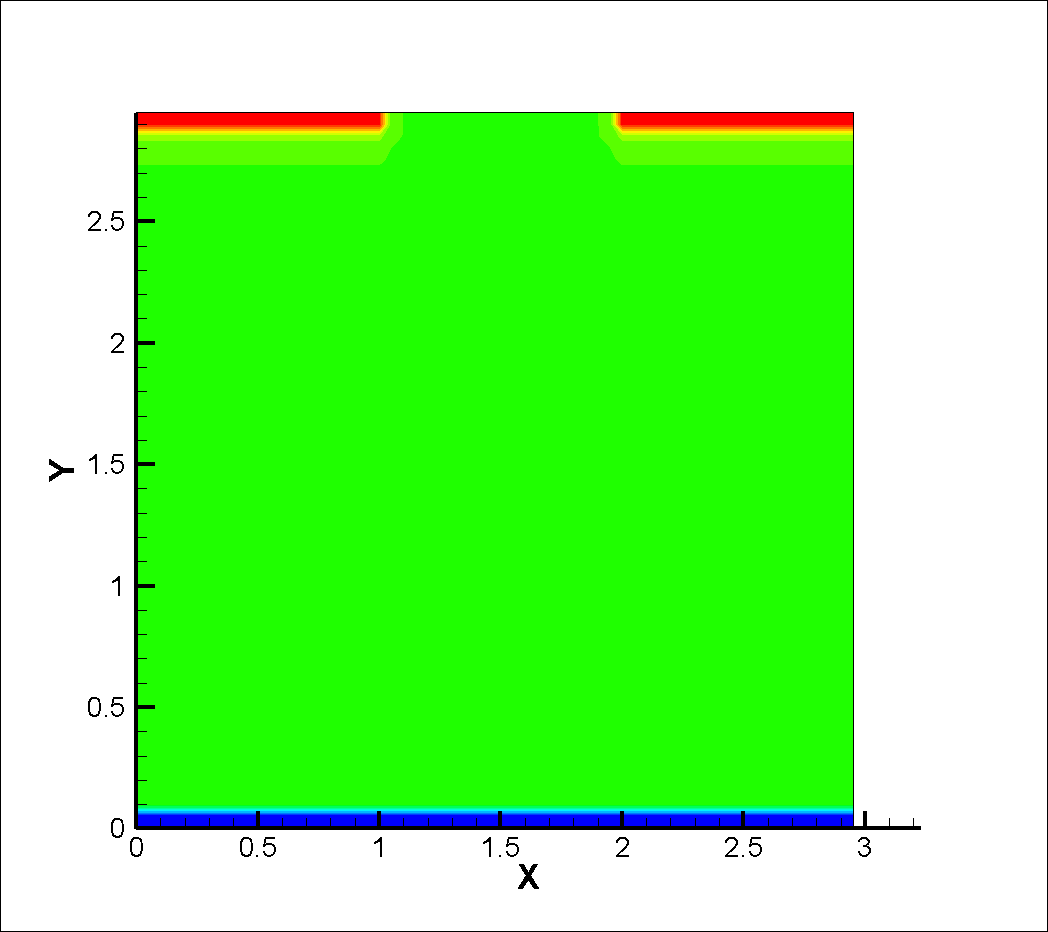
\includegraphics[width=5cm,height=5cm]{test2_1Sg}
\end{center}
\begin{center}
 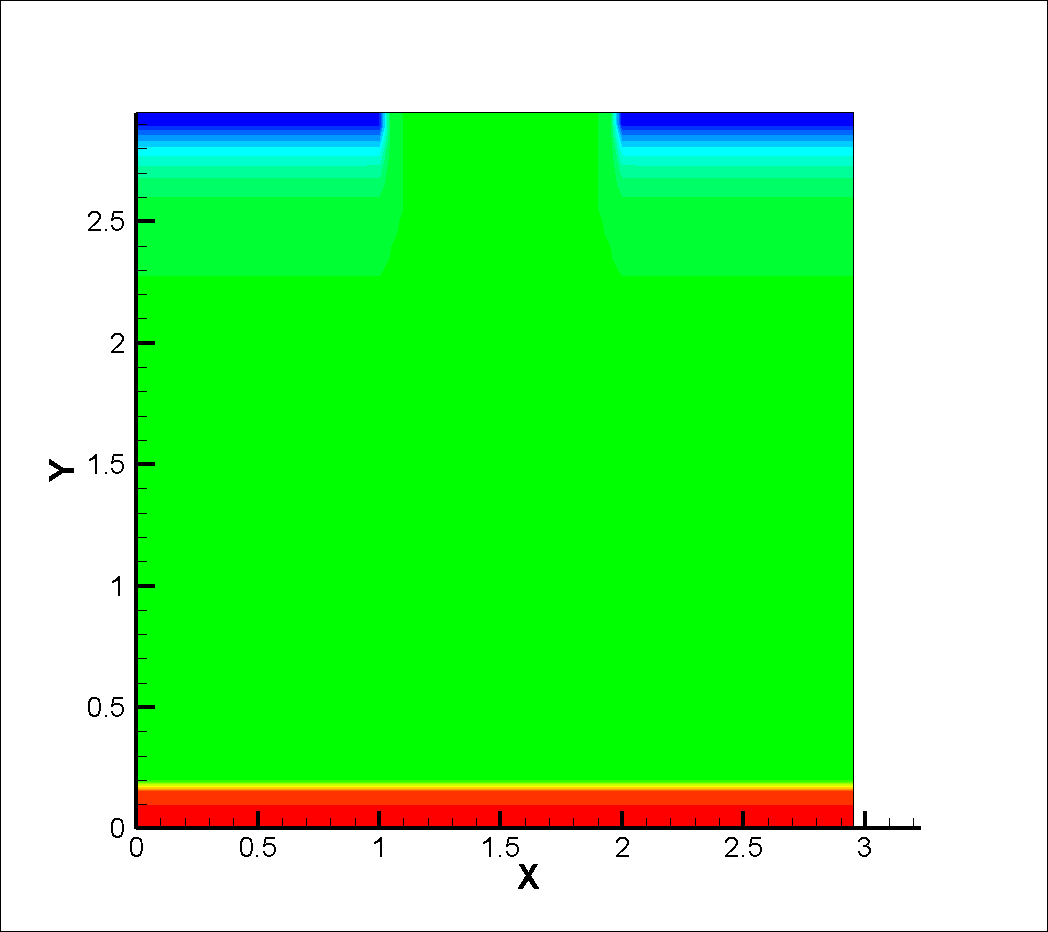
\includegraphics[width=5cm,height=5cm]{test2_2Sw}
 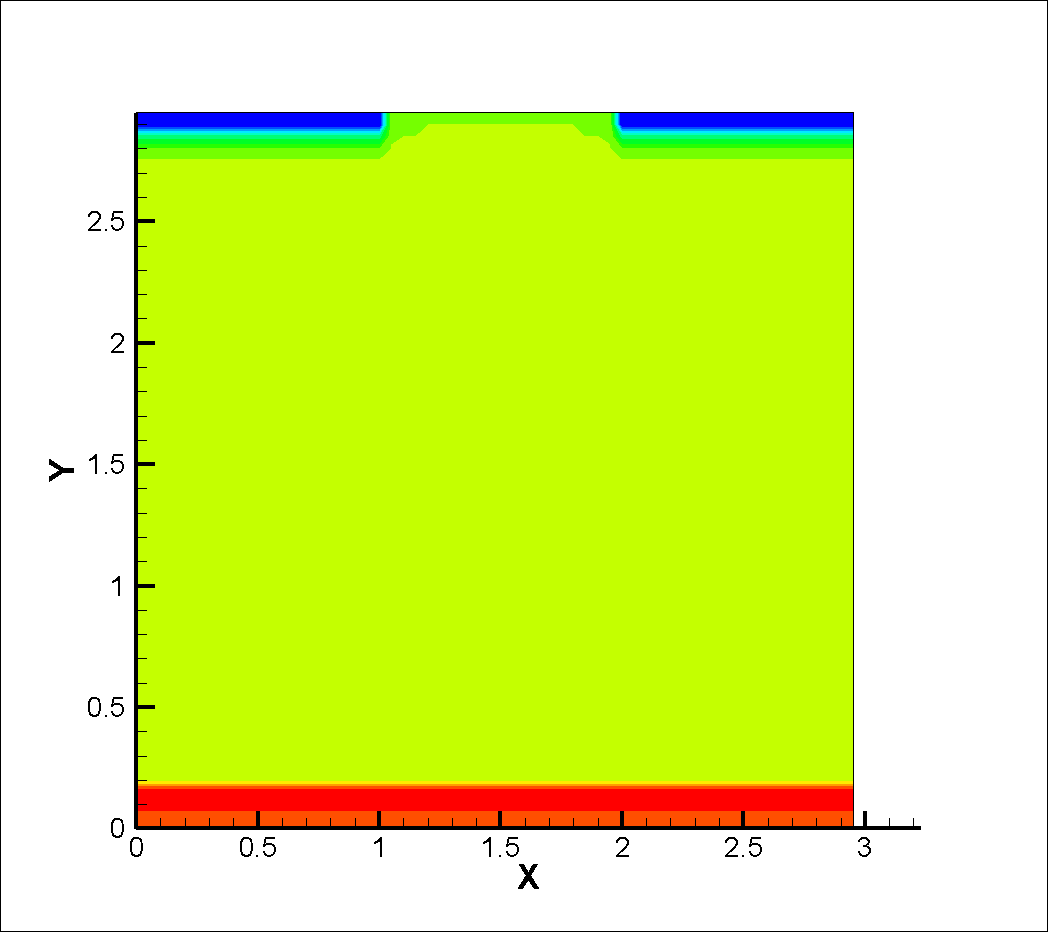
\includegraphics[width=5cm,height=5cm]{test2_2Sn}
 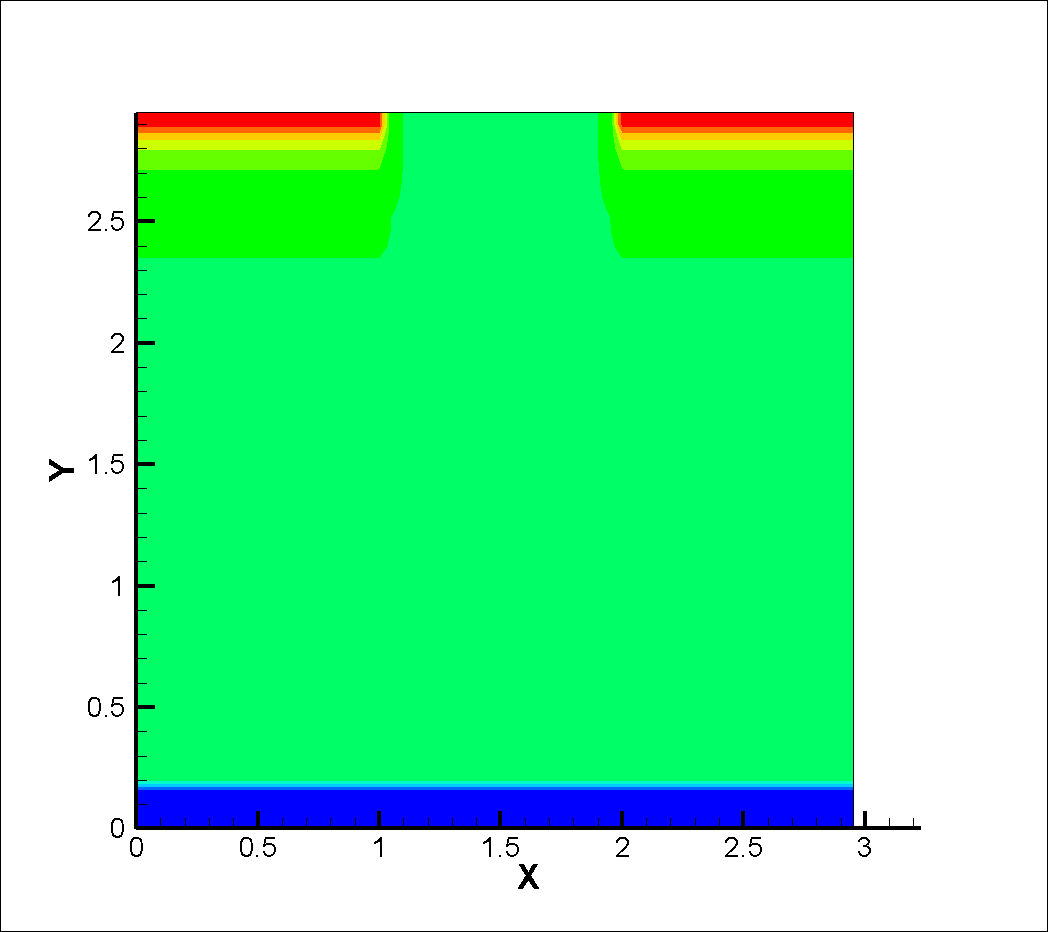
\includegraphics[width=5cm,height=5cm]{test2_2Sg}
\end{center}
\begin{center}
 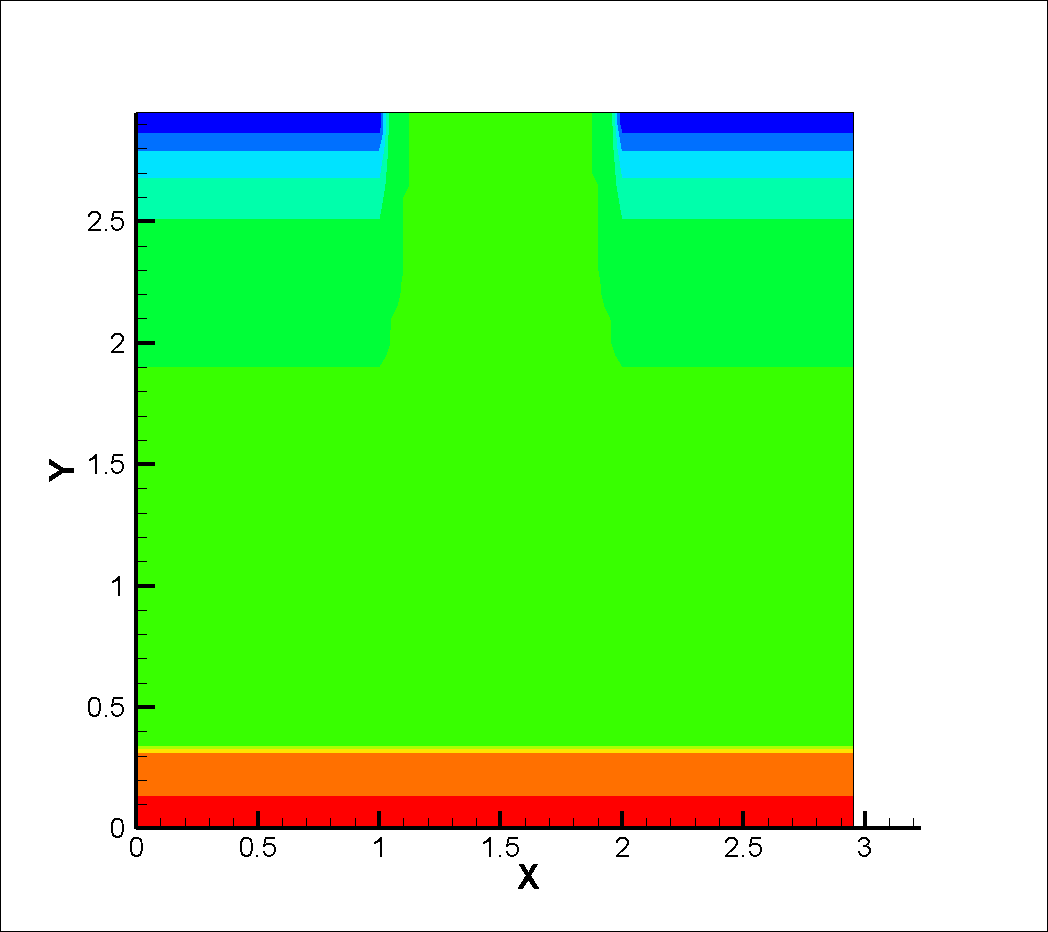
\includegraphics[width=5cm,height=5cm]{test2_3Sw}
 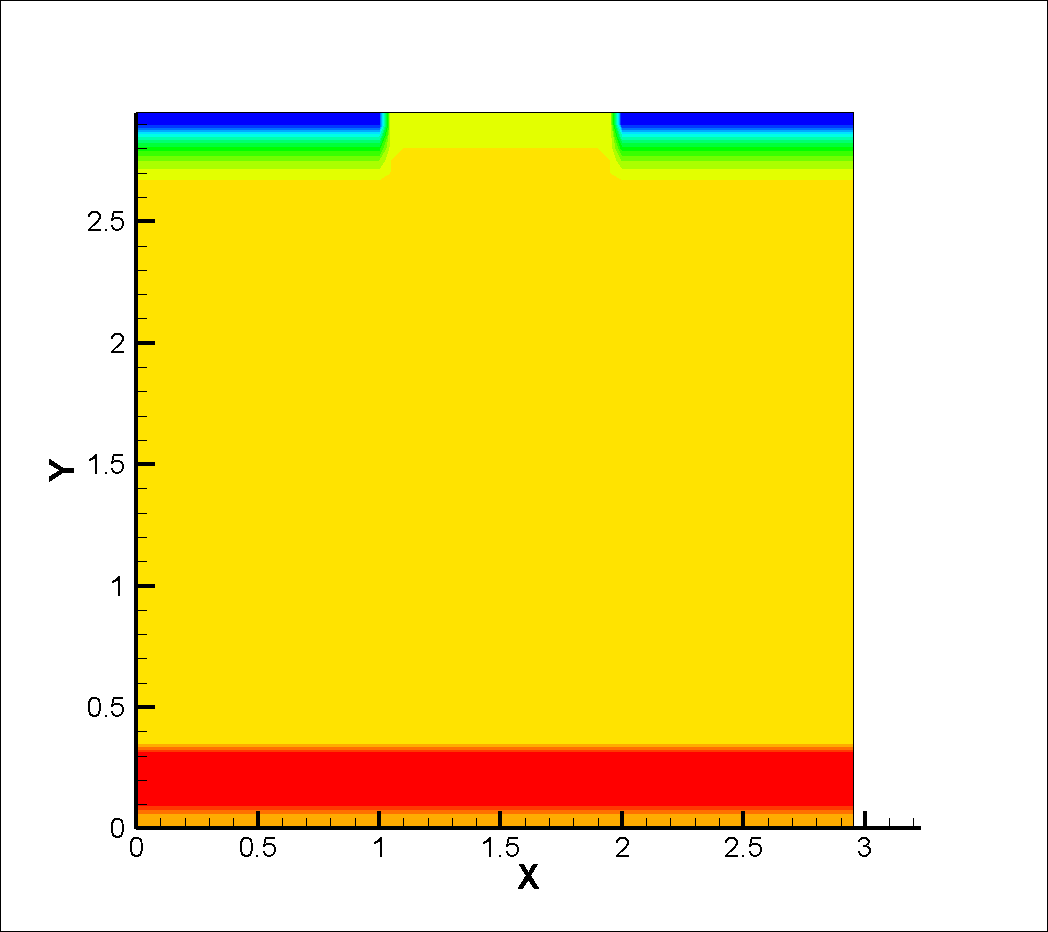
\includegraphics[width=5cm,height=5cm]{test2_3Sn}
 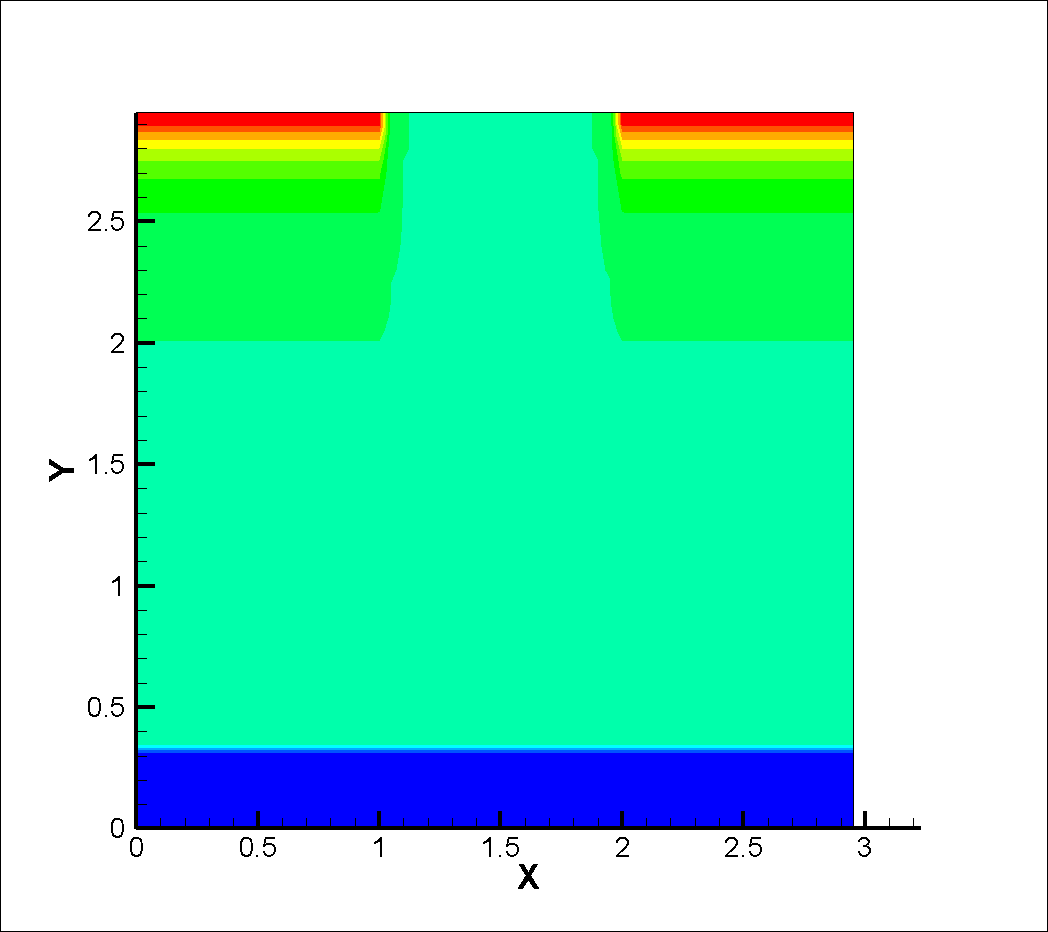
\includegraphics[width=5cm,height=5cm]{test2_3Sg}
\end{center}
\begin{center}
 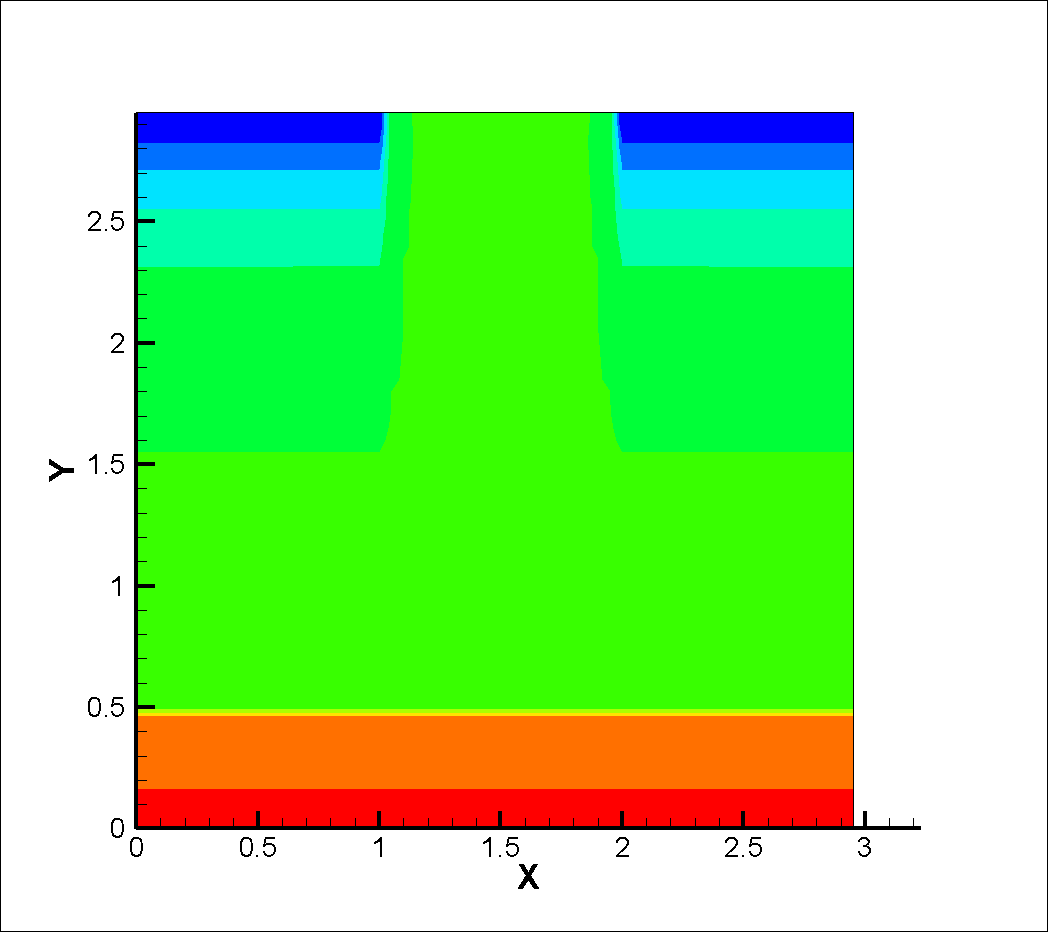
\includegraphics[width=5cm,height=5cm]{test2_4Sw}
 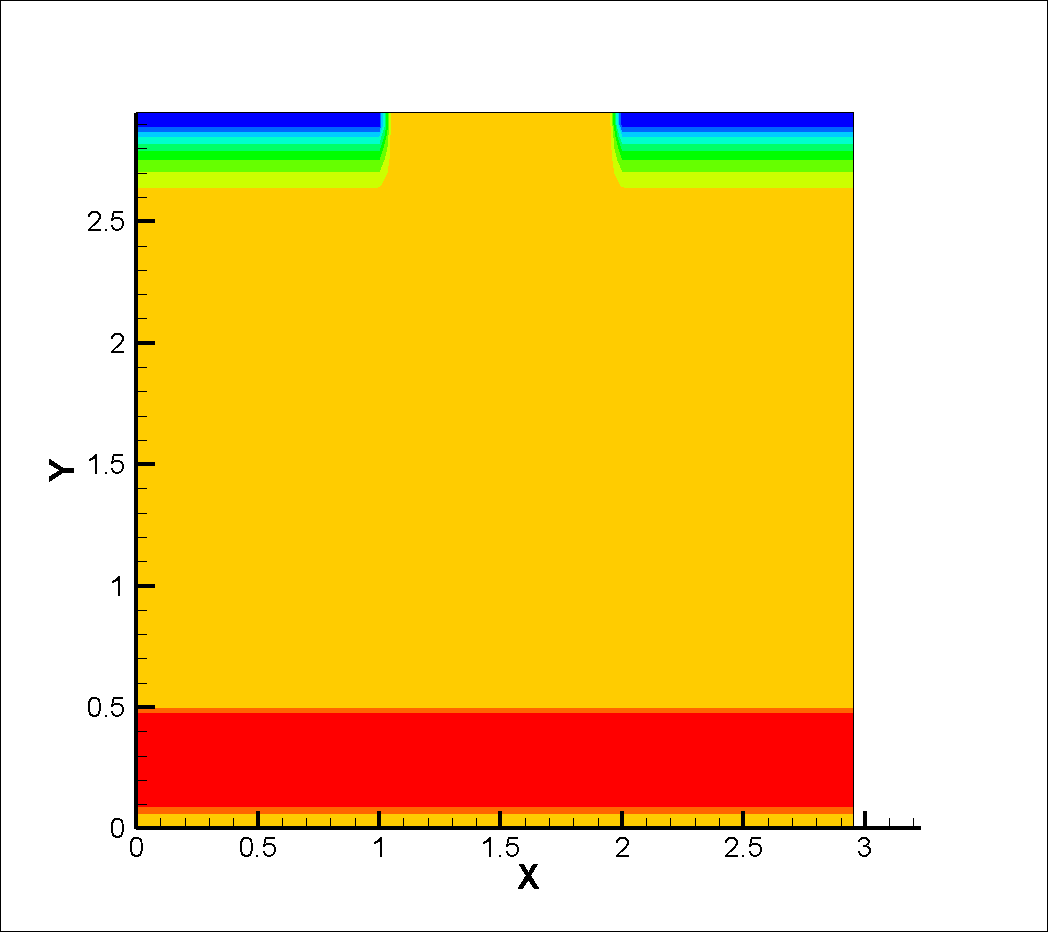
\includegraphics[width=5cm,height=5cm]{test2_4Sn}
 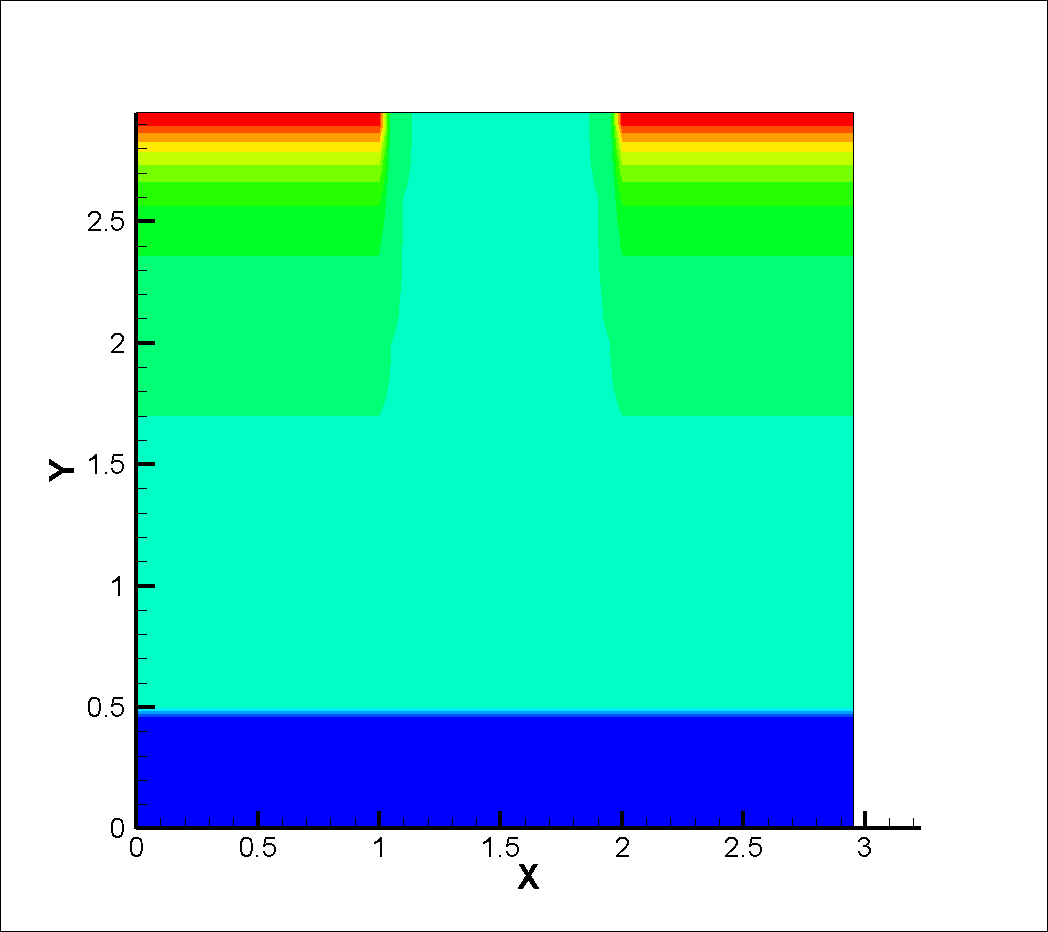
\includegraphics[width=5cm,height=5cm]{test2_4Sg}
\end{center}

Из представленных графиков видно, что вода проникает через отверстие в область и накапливается 
у дна резервуара, газ скапливается у непроницаемой части верхней границы и выходит через отверстие 
наружу, нефть частично концентрируется у нижнего края области, но, вытесняемая водой,
 понемногу поднимается к отверстию из средних слоев.  

\subsection{Двумерная задача нефтедобычи}
Рассматриваем трехмерную область пористой среды, имеющую форму параллелепипеда. Считаем,
что имеет место независимость распределений от глубины, т.е. задача ставится, как двумерная. 
Действием силы тяжести и капиллярных сил пренебрегаем. Пористость и
абсолютная проницаемость породы постоянны во всем объеме. Параметры модели такие же, как
в первой тестовой задаче. Во всей области задаем следующее 
начальное распределение: $S_w=0.4$,\; $S_n=0.35$,\; $S_g=0.25$, 
$P_w=P_\text{атм}$. Граничную поверхность считаем непроницаемой.

Пусть размер области -- $Nx\cdot Ny$.
Задаем по четыре нагнетательные и добывающие скважины в точках со следующими координатами.
Нагнетательные: $(N_x/4, N_y/4)$, $(3N_x/4, N_y/4)$, $(3N_x/4, 3N_y/4)$, $(N_x/4, 3N_y/4)$.
Добывающие: $(N_x/2, N_y/4)$, $(N_x/4, N_y/2)$, $(N_x/2, 3N_y/4)$, $(3N_x/4, N_y/2)$.
Радиус скважин пропорционален размеру области.
В точках, отведенных под скважины, в уравнении неразрывности для каждой из фаз 
в правой части добавляем слагаемое $q_i$,\; $i=w,n,g$.
Для простоты считаем, что на нагнетательных скважинах $q_i=const$,\; $i=w,n,g$, 
а на добывающих $q_i=q_i(S_i)$,\; $i=w,n,g$.

В результате расчетов получены следующие распределения давления и траекторий частиц фаз:
\begin{center}
 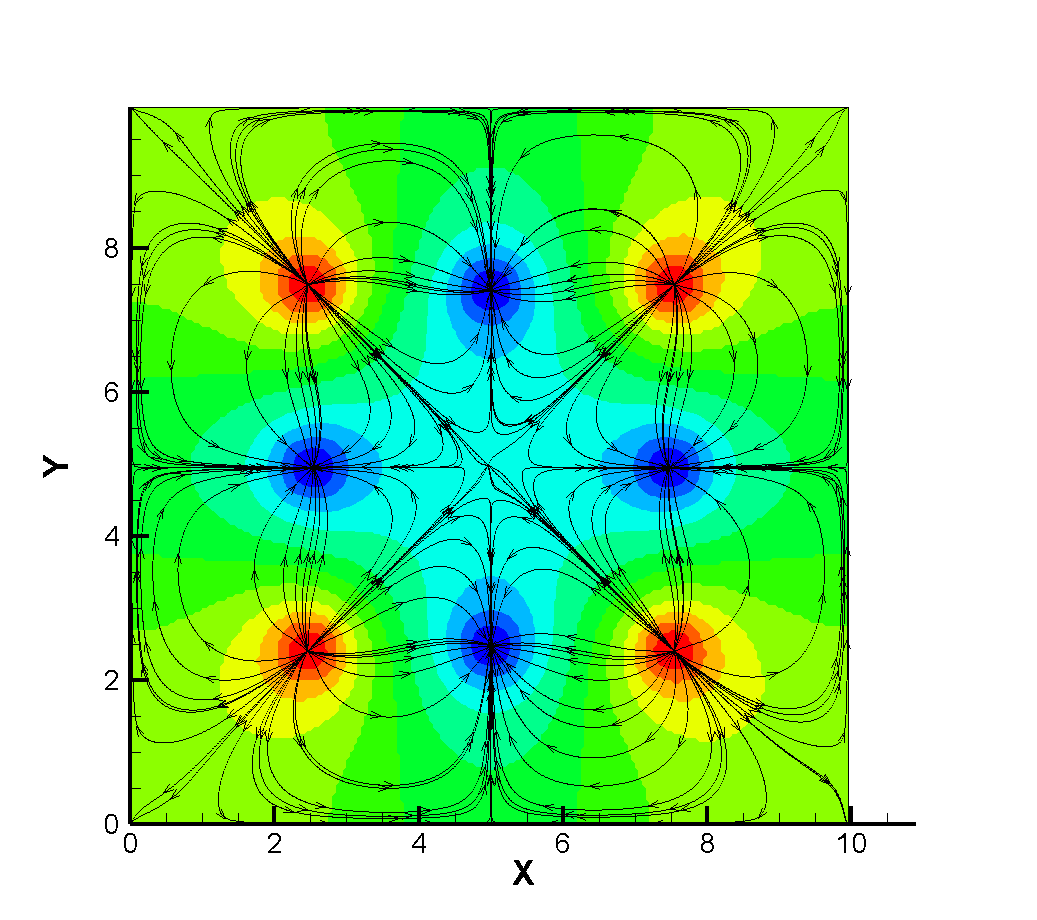
\includegraphics[width=15.5cm,height=14.5cm]{test3}
\end{center}
Все три фазы движутся по одним и тем же траекториям: от нагнетательных скважин к 
добывающим. Распределение давлений с течением времени не меняет очертаний.
